% !TeX spellcheck = da_DK
\subsection{Referencespænding til offset}\label{subsec:Spaendingsref}
\subsubsection{Teori og design}
Offsetjusteringen skal forsynes med en konstant spænding, da denne er sammenligningsgrundlag ift. inputsignalet. Denne konstante spænding kaldes en referencespænding og består af en spændingsforsyning, en modstand og en referencediode. Der anvendes en referencediode af typen LM385, som både findes som $1.2$V og $2.5$V. Et eksempel på en opsætning af en spændingsreference kan ses på \figref{fig:Spaendingsreference}.

\begin{figure}[H]
	\centering
	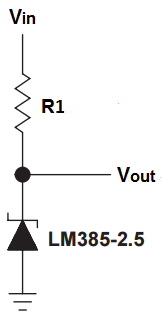
\includegraphics[scale=0.7]{figures/cProblemloesning/ReferenceEksempel.PNG}
	\caption{På figuren ses et eksempel på en opsætning af et kredsløb for en spændingsreference med referencedioden LM$385$. Modstanden $R1$ afhænger af $V_{in}$, $V_{out}$ samt strømforbruget fra LM$385$. \textit{(Revideret)} \cite{Instruments2005}}
	\label{fig:Spaendingsreference}
\end{figure}

\noindent For at udregne værdien af modstanden R$1$ på \figref{fig:Spaendingsreference} anvendes følgende generelle formel:
\begin{equation}\label{eq:udregning_modstand}
R1 = \dfrac{V_{forsyning} - V_{Reference}}{I_{Z}}
\end{equation}
\noindent Hvor $V_{forsyning}$ er forsyningsspændingen, der sendes ind i kredsløbet, $V_{Reference}$ er den referencespænding, der skal sendes ud af systemet, og $I_{Z}$ er strømforbruget fra de komponenter, som er i referencespændingskredsløbet. \\
Først udregnes R$1$ for referencespændingen. $V_{forsyning}$ er de $5.5$V, der forsynes med fra spændingsforsyningen, og $V_{Reference}$ er $2.5$V. I kredsløbet for offsettet indgår en operationsforstærker (TL$081$), der har en maksimal biasstrøm på $10$nA \cite{Corporation1995}. Referencedioden har et arbejdsområde mellem $20\mu$A til $20m$A og for at sikre, at der er strøm nok til referencedioden, er den sat til at bruge $200\mu$A \cite{Instruments2005}. Dermed kan strømforbruget $I_{Z}$ udregnes som summen af de to biasstrømme. Alle de kendte værdier indsættes i formlen:
\begin{equation}
R1 = \frac{5.5V - 2.5V}{0.2mA + 10nA} = 14999.2500\Omega \approx 15K\Omega
\end{equation}  
Da offsettet i accelerometeret er på $1.6325$V, jævnfør bilag \ref{Sec_Pilot_Data} på side \pageref{Sec_Pilot_Data}, skal referenceværdien ligeledes være $1.6325$V. For at opnå denne referenceværdi benyttes en spændingsdeler efter referencedioden, der leverer $2.5$V. Den generelle formel for en spændingsdeler er: 
\begin{equation} \label{eq:Spaendingsdeler}
V_{out} = V_{in} \cdot \dfrac{R3}{R2 + R3}
\end{equation}
\noindent R$2$ i \eqref{eq:Spaendingsdeler} bliver valgt til at være $10$K$\Omega$. Derudover er $V_{out}$ lig $1.6325$V og $V_{in}$ er $2.5$V. Ligningen kommer til at se således ud: 
\begin{eqnarray}
1.6325V = 2.5 \cdot \dfrac{R3}{10000\Omega + R3} \\
R3 = 18818.4438\Omega \approx 18820\Omega
\end{eqnarray}
\noindent På \figref{fig:Spaendingsreference_offset} ses designet af spændingsreferencen med spændingsdeler. 
\begin{figure}[H]
	\centering
	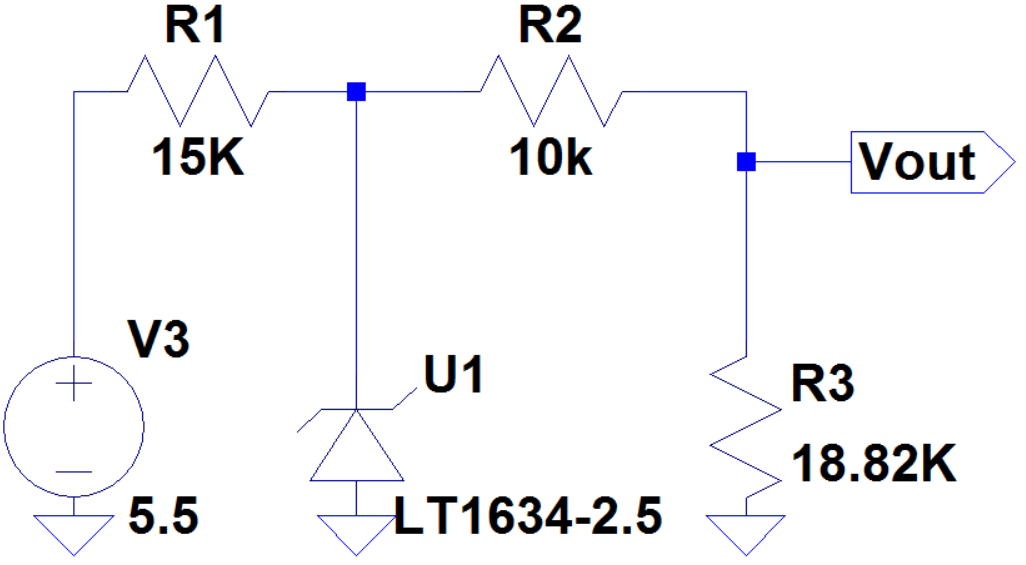
\includegraphics[scale=.5]{figures/cProblemloesning/OffsetSpaendingsRef2.PNG}
	\caption{På figuren ses designet af kredsløbet for en spændingsreference til offsettet. Først ses opbygningen af en spændingsreference efterfulgt af en spændingsdeler, som medfører, at outputtet fra spændingsreferencen på $2.5$V bliver til $1.6325$V.}
	\label{fig:Spaendingsreference_offset}
\end{figure}

\subsubsection{Simulering}
Der foretages en simulering i LTspice af spændingsreferencen og spændingsdeleren for at undersøge, om de opstillede krav opfyldes. På \figref{fig:Spaendingsreference_offset_sim} ses simuleringen af spændingsreferencen og spændingsdeleren.

\begin{figure}[H]
	\centering
	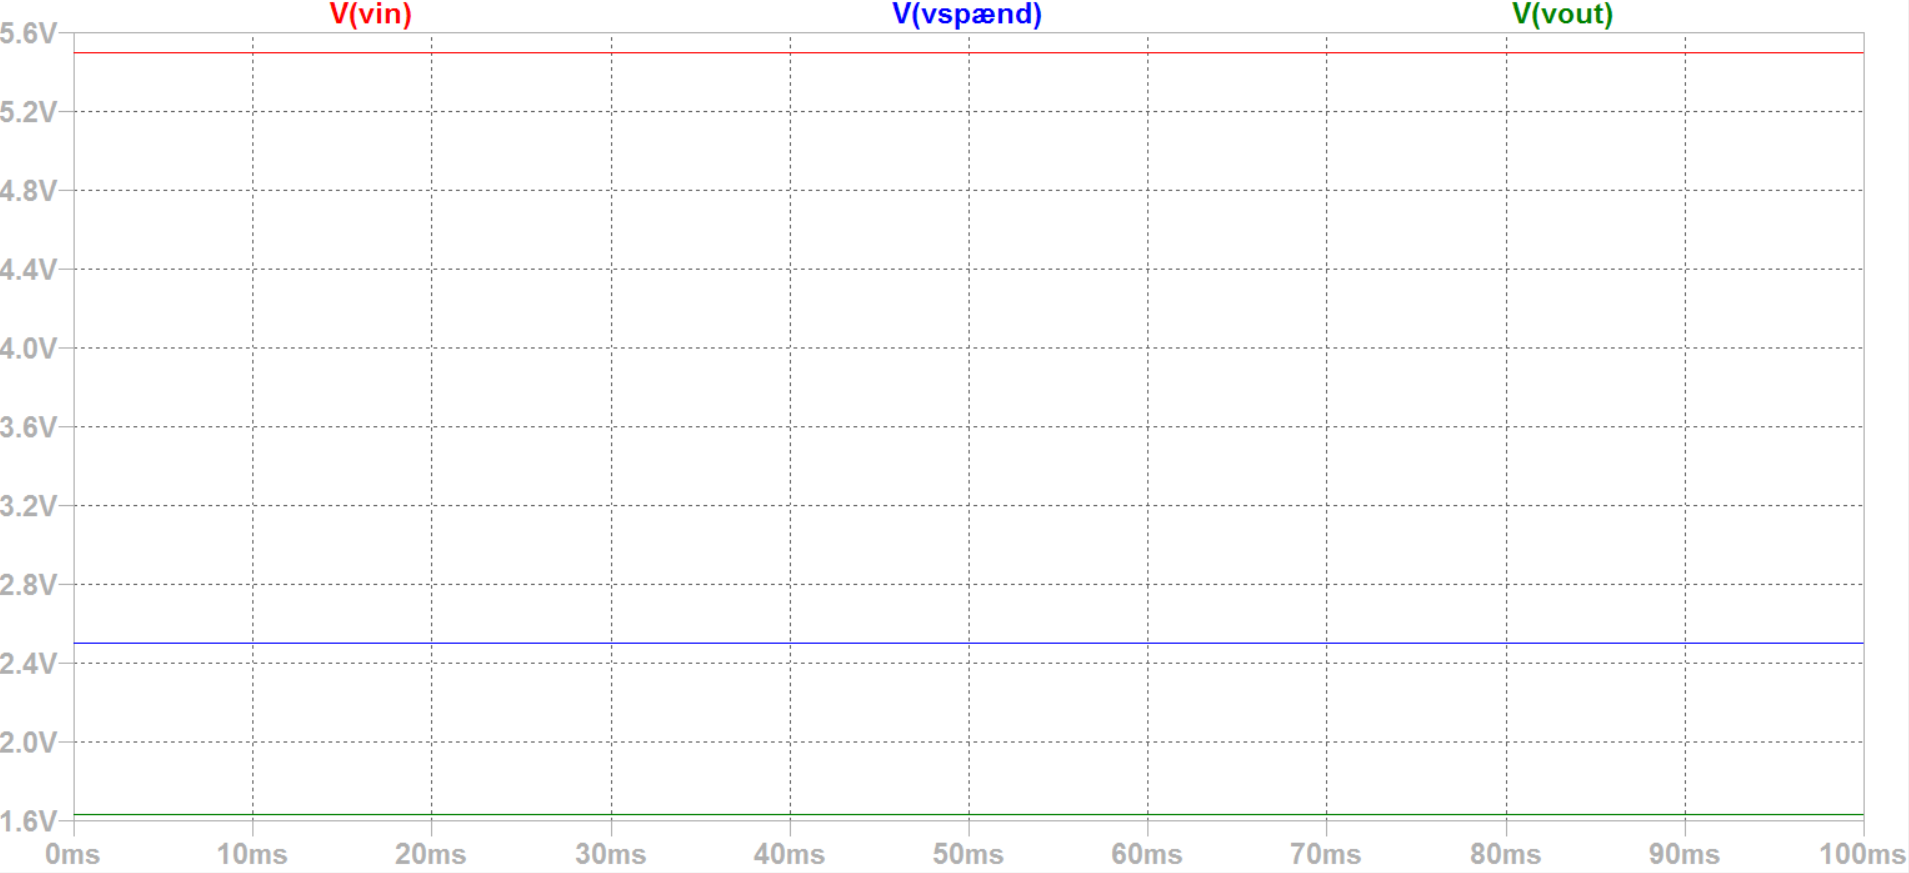
\includegraphics[scale=.37]{figures/cProblemloesning/Reference_sim_off.PNG}
	\caption{På figuren ses en simulering af referencespændingen med spændingsdeleren. Der ses, at inputtet er $5.50$V (rød), outputtet fra spændingsreferencen er $2.50$V (blå) og outputtet fra spændingsdeleren er ca. $1.65$V (grøn).}
	\label{fig:Spaendingsreference_offset_sim}
\end{figure}

\noindent Resultatet af simuleringen kan ses i \tableref{Tab:SpaendigsRef_offset}:
\begin{table}[H]
	\centering
	\begin{tabular}{|l|l|l|l|}\hline
		& \textit{\begin{tabular}[c]{@{}l@{}}Forventet\\outputsignal\end{tabular}} & \textit{\begin{tabular}[c]{@{}l@{}}Målte\\outputsignal\end{tabular}} & \textit{Afvigelse} \\ \hline
		\textit{\begin{tabular}[c]{@{}l@{}}Input fra\\spændingsforsyning\end{tabular}}      & $5.5$V             &   $5.5$V      &   $0\%$         \\ \hline
		\textit{\begin{tabular}[c]{@{}l@{}}Output fra\\spændingsreference\end{tabular}}     & $2.5$V             &  $2.5007$V    &   $0.03 \%$    \\ \hline
		\textit{\begin{tabular}[c]{@{}l@{}}Output fra\\spændingsdeler\end{tabular}}         & $1.6325$V          &  $1.6330$V    &   $0.03 \%$     \\ \hline
	\end{tabular}
	\caption{I tabellen ses resultaterne fra simuleringen i LTspice af spændingsreferencen med spændingsdeleren til offsettet.}
	\label{Tab:SpaendigsRef_offset}
\end{table}
\noindent I \tableref{Tab:SpaendigsRef_offset} fremgår det, at der er en afvigelse mellem det forventede output og det simulerede output. Der ses, at afvigelserne ligger inde for tolerancerne, jævnfør afsnit \ref{Ref_Offset_Afs}, side \pageref{Ref_Offset_Afs}, og accepteres derfor til implementeringen.

\subsubsection{Implementering og test}\label{spaendingsref_resultat}
%I implementeringen arbejdes der med reelle komponenter. Derfor antages det, at der kan være afvigelser fra resultaterne imellem testen med ideelle komponenter i dette afsnit og testen med reelle komponenter i simuleringen. \\
Der ses på \figref{fig:Spaendingsreference_offset}, at der skal benyttes tre modstande på hhv. $15$K$\Omega$, $10$K$\Omega$ og $18.82$K$\Omega$ til opbygningen af spændingsreferencen og spændingsdeleren til offsettet. Der findes ikke en $18.82$K$\Omega$, hvorfor en $18$K$\Omega$ modstand i serie med en $820\Omega$ modstand benyttes. Disse måles inden testen, hvilket fremgår i \tableref{Tab:modstand_offset}.

\begin{table}[H]
	\centering
	\begin{tabular}{|l|l|l|}
		\hline
		\textit{Teoretisk} & \textit{Ved måling} & \textit{Afvigelse} \\ \hline
		$15$K$\Omega$       & $15.0020$K$\Omega$      & $0.01$\%               \\ \hline
		$10$K$\Omega$       & $10.0036$K$\Omega$ & $0.04$\%               \\ \hline
		$18$K$\Omega$       & $17.9653$K$\Omega$ & $0.19$\%               \\ \hline		
		$820\Omega$         & $818.0800\Omega$     & $0.23$\%               \\ \hline
		$R_{eq}$ af $18$K$\Omega$ + $820\Omega$ = $18.82$K$\Omega$ & $18.8734$K$\Omega$ & $0.28\%$ \\ \hline
	\end{tabular}
	\caption{I tabellen ses, at alle fire modstande afviger fra deres teoretiske værdi, hvilket er forventet af reelle komponenter, som også vil have en effekt på afvigelsen af den ækvivalente værdi for $18$K$\Omega$ + $820\Omega$.}
	\label{Tab:modstand_offset}
\end{table}
\noindent Herefter implementeres kredsløbet. Til aflæsning af spændingsniveauerne anvendes et multimeter. De aflæste resultater fremgår i \tableref{Tab:SpaendingsRef_offset_test}.
\begin{table}[H]
\centering
\begin{tabular}{|l|l|l|l|} \hline
                              & \textit{\begin{tabular}[c]{@{}l@{}}Forventet\\outputsignal\end{tabular}} & \textit{\begin{tabular}[c]{@{}l@{}}Målte\\outputsignal\end{tabular}} & \textit{Afvigelse} \\ \hline
\textit{\begin{tabular}[c]{@{}l@{}}Input fra\\spændingsforsyning\end{tabular}}       & $5.5$V    & $5.550$V  & $0.91 \%$ \\ \hline
\textit{\begin{tabular}[c]{@{}l@{}}Output fra\\spændingsreference\end{tabular}}      & $2.5$V    & $2.499$V  & $0.04 \%$ \\ \hline
\textit{\begin{tabular}[c]{@{}l@{}}Output fra\\spændingsdeler\end{tabular}}          & $1.6325$V & $1.6307$V & $0.11 \%$ \\ \hline
\end{tabular}
\caption{I tabellen ses en oversigt over de forventede og målte outputsignaler fra testen for spændingsreferencen og spændingsdeleren til offsetjustering.}
\label{Tab:SpaendingsRef_offset_test}
\end{table}
%Ud fra \tableref{Tab:SpaendingsRef_offset_test} ses det, at afvigelserne for inputtet fra spændingsreferencen har en lidt større afvigelse end de andre. Dette kan skyldes, at spændingsforsyningen ikke er ideel og derfor kan variere lidt i dens outputspænding. Variationen fra spændingsforsyningen vil ikke have en indflydelse, hvis den ikke varierer mere end det målte. Outputtet fra spændingsreferencen accepteres, da afvigelsen er på $0.04 \%$. Det samme gælder for outputtet af spændingsdeleren, hvor afvigelsen er på $0.18 \%$. 
\noindent Der ses ud fra resultaterne i \tableref{Tab:SpaendingsRef_offset_test}, at spændingsreferencen samt spændingsdeleren overholder kravene fra afsnit \ref{Ref_Offset_Afs} på side \pageref{Ref_Offset_Afs}. Derudover ligger afvigelserne indenfor tolerancerne. \\
Outputimpedansen overholder ikke kravet, da den er:
\begin{equation}
R_{eq} = \dfrac{(R2 \cdot R3)}{R2 + R3} \Longrightarrow \dfrac{10000 \cdot 18820}{10000 + 18820} = 6530.19\Omega \approx 6.53K\Omega
\end{equation}
\noindent Da inputimpedansen i den inverterende kanal i operationsforstærkeren i offsetjusteringen har en indgangsimpedans på $100$K$\Omega$, vil forholdet mellem output- og inputimpedans i koblingen være problematisk. Der vil dannes en spændingsdeling imellem R$3$ og den pågældende modstand, som sidder inden den inverterende kanal. Dermed vil signalet variere alt efter inputsignalet til operationsforstærkeren i offsetjusteringens ikke-inverterende kanal. Løsningen på problematikken i denne kobling er, at indsætte en buffer, som er beskrevet i bilag \ref{Bilag:Pilotforsoeg}, side \pageref{Bilag:Pilotforsoeg}. \cite{Schaumann2014} Signalet fra spændingsdeleren sendes ind i bufferens ikke-inverterende kanal, hvorfor outputimpedansen ikke er relevant, da denne kanal har en indgangsimpedans på $10^{12}\Omega$. Herved kan blokken accepteres og benyttes i det samlede kredsløb.